\subsection{Understanding Wavelength Units on a Smith Chart!}

\begin{tcolorbox}[colback=gray!10, colframe=black, title=E9G11]
In what units are the wavelength scales on a Smith chart calibrated? 

\begin{enumerate}[label=\Alph*.]
    \item In fractions of transmission line electrical frequency
    \item \textbf{In fractions of transmission line electrical wavelength}
    \item In fractions of antenna electrical wavelength
    \item In fractions of antenna electrical frequency
\end{enumerate} \end{tcolorbox}

\subsubsection*{Related Concepts}

To answer this question, it is essential to understand what a Smith chart is and how it is used in radio communication and electronics. A Smith chart is a graphical representation used for calculating impedance, reflection coefficients, and for the design of matching networks in RF (radio frequency) circuits.

The key aspect of the Smith chart is that it represents the relationships between the impedance and the wavelength along a transmission line. The scales of the Smith chart are calibrated in fractions of the electrical wavelength because these fractions directly relate to the behavior of signals travelling down transmission lines, specifically how the impedance changes with respect to the wavelength of the signal.

\subsubsection*{Concepts Required to Answer the Question}

1. \textbf{Transmission Line Theory:}: Understanding of how transmission lines work, including concepts like standing waves, impedance, and reflections.
2. \textbf{Wavelength:}: A solid grasp of the definitions and implications of wavelength in electrical terms, particularly how it relates to frequency and the speed of light.

To find these relationships, the following formula is helpful:

\[
\text{Wavelength} (\lambda) = \frac{v}{f}
\]

where \( v \) is the velocity of the signal in the medium (approximately the speed of light in vacuum for RF applications) and \( f \) is the frequency of the signal. 

Because the Smith chart is primarily used for RF applications and not for antenna directivity or frequency calibration, its scales are focused on transmission line parameters.

\subsubsection*{Illustration}

Below is a diagram illustrating the relationship between frequency, wavelength, and the use of a Smith chart:

\begin{center}
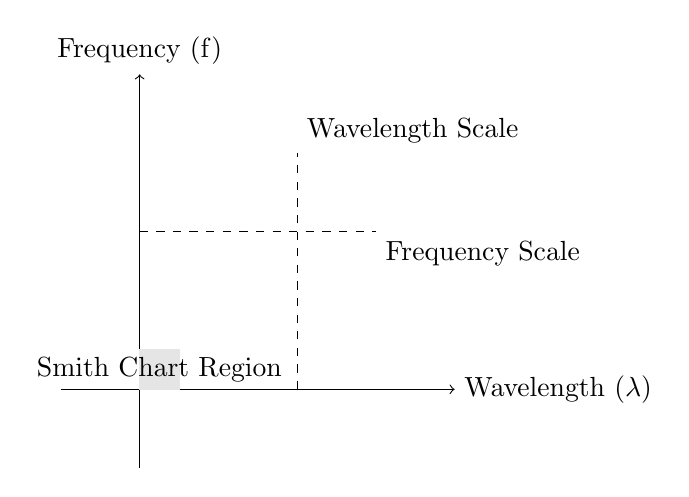
\begin{tikzpicture}
    \draw[->] (-1,0) -- (4,0) node[right] {Wavelength (\(\lambda\))};
    \draw[->] (0,-1) -- (0,4) node[above] {Frequency (f)};
    
    \draw[dashed] (2,0) -- (2,3) node[above right] {Wavelength Scale};
    \draw[dashed] (0,2) -- (3,2) node[below right] {Frequency Scale};
    
    \filldraw[gray!20] (0,0) rectangle (0.5,0.5);
    \node at (0.25,0.25) {Smith Chart Region};
\end{tikzpicture}
\end{center}
